\chapter{Lecture 29 - Fourier Series in Two Variables}
\label{ch:lec29}
\section{Objectives}
\begin{itemize}
\item Present Fourier series expansions in two (or more) independent variables.
\item Show an example application in the solution to the heat equation in two spatial dimensions.
\end{itemize}
\setcounter{lstannotation}{0}

\section{Fourier Series Expansion in Two Variables}

Consider the function $f(x,y), \ 0<x<a, \ 0<y<b$.  Suppose I want to represent the function in the form of a \emph{double} Fourier series as follows:

\begin{equation}
f(x,y) = \sum\limits_{m=1}^{\infty}\sum\limits_{n=1}^{\infty} A_{mn}\sin{\frac{m\pi y}{a}} \sin{\frac{n \pi x}{b}}
\label{eq:double-fourier}
\end{equation}

\begin{enumerate}

\item Should we expect this to be possible?  Answer: of course!  Fourier series have shown themselves to be a perfectly adequate tool for representing a variety of functions.  There is no problem in adding another spatial dimension

\item How will we determine the appropriate values for $A_{mn}$?  Answer: we will multiply both sides by orthogonal function\underline{s} and integrate, as usual.\marginnote{Again, these sets of functions---$\sin{\sfrac{m \pi x}{a}}$ and $\sin{\sfrac{n \pi y}{b}}$---are orthogonal with respect to a weight function $p(x)=1$ and we should not forget it even if we leave it out of the equations and fail to mention it in the discussion.}

\end{enumerate}
\begin{multline*}
\int_0^b \int_0^a f(x,y) \sin{\frac{m^{\prime} \pi x}{a}} \sin{\frac{n^{\prime} \pi y}{b}} \ dx \ dy = \cdots \\ \int_0^a \int_0^b A_{mn}\sin{\frac{m \pi x}{a}} \sin{\frac{n \pi y}{b}}\sin{\frac{m^{\prime} \pi x}{a}} \sin{\frac{n^{\prime} \pi y}{b}} \ dx \ dy
\end{multline*}
where, if $m^{\prime}=m$ and $n^{\prime} = n$ then:\marginnote{Of course, if $m^{\prime}\ne m$ or $n^{\prime} \ne n$ then the respective integral is zero by orthogonality.}
\begin{multline*}
\int_0^b \int_0^a f(x,y) \sin{\frac{m^{\prime} \pi x}{a}} \sin{\frac{n^{\prime} \pi y}{b}} \ dx \ dy = \cdots \\ A_{mn} \underbrace{\left[\int_0^a \sin{(\frac{m \pi x}{a})}^2 \ dx \right]}_{=\frac{a}{2}} \underbrace{ \left[ \int_0^b \sin{(\frac{n \pi y}{b})}^2 \ dy \right]}_{=\frac{b}{2}}
\end{multline*}
So that
\begin{equation}
A_{mn} = \frac{4}{a b} \int_0^b \int_0^a f(x,y) \sin{\frac{m \pi x}{a}} \sin{\frac{n \pi y}{b}} \ dx \ dy
\label{eq:double-fourier-coeff}
\end{equation}

\section{MATLAB Implementation}
Implementing this expansion in MATLAB is mostly straight-forward.  We will start by defining parameters:
\marginnote{

\vspace{4.0 cm}

\ref{lst:ann29-1-1} Here we use a \lstinline[style=myMatlab]{switch...case} selection structure.  For the in-class demonstration I like to choose between different functions for which the double Fourier expansion will be used.  The parameter \lstinline[style=myMatlab]{ex_select} is set to either 1 or 2; the \lstinline[style=myMatlab]{case} statements allow me to assign a function handle t \lstinline[style=myMatlab]{f} accordingly.  The \lstinline[style=myMatlab]{otherwise} statement allows me to deal gracefully deal with having specified an invalid value for \lstinline[style=myMatlab]{ex_select}.

}
\begin{lstlisting}[name=lec29-ex1, style=myMatlab]
clear
clc
close 'all'

%% Parameters
a = 4;
b = 3;

N = 20;

ex_select = 1;
% 1 smooth
% 2 not smooth

switch ex_select  /*!\annotation{lst:ann29-1-1}!*/
    case 1
        f = @(x,y) x.*(a-x).*y.*(b-y);
        
    case 2
       f = @(x,y) ex1(x,y,a,b);
       
    otherwise
        error('Invalid Example Choice!');
end
\end{lstlisting}

Next we will visualize the function that we hope to represent with a double Fourier series.

\begin{lstlisting}[name=lec29-ex1,style=myMatlab]
Nx = 250;
Ny = 250;

X = linspace(0,a,Nx);
Y = linspace(0,b,Ny);

[XX,YY] = meshgrid(X,Y);

figure(1)
surf(XX,YY,f(XX,YY),'edgecolor','none');
title('f(x,y)','fontsize',16,'fontweight','bold');
xlabel('X','fontsize',14,'fontweight','bold');
ylabel('Y','fontsize',14,'fontweight','bold');
zlabel('f(X,Y)','fontsize',14,'fontweight','bold');
set(gca,'fontsize',12,'fontweight','bold');


\end{lstlisting}

\begin{figure}[h!]
\subfloat[]{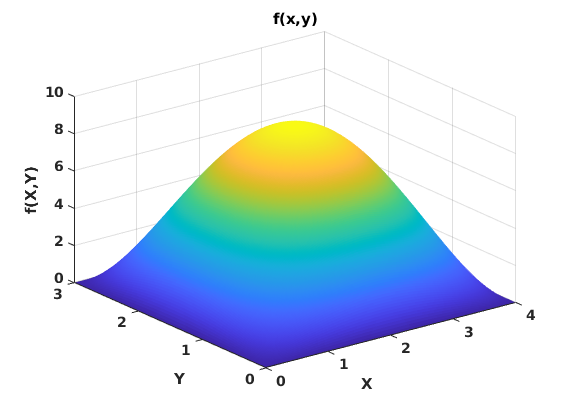
\includegraphics[width=2in]{lec29-fx1.png}}
\subfloat[]{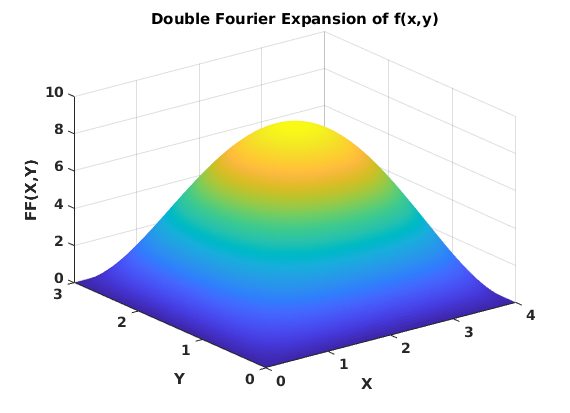
\includegraphics[width=2in]{lec29-fx1-dfexp.png}} \\
\subfloat[]{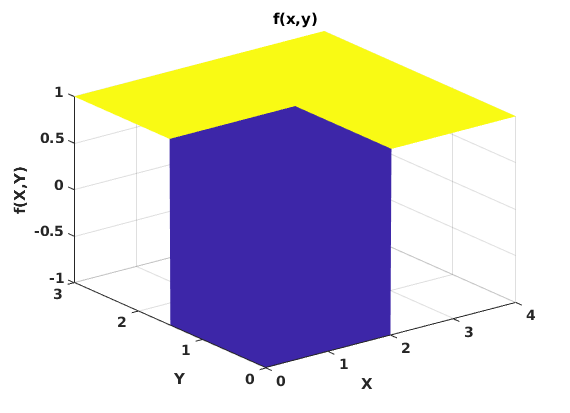
\includegraphics[width=2in]{lec29-fx2.png}}
\subfloat[]{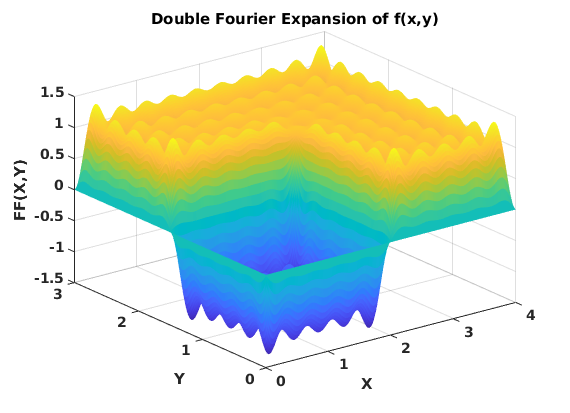
\includegraphics[width=2in]{lec29-fx2-dfexp.png}}
\label{fig:lec29-dfexp}
\caption{Plots of example functions and their double Fourier series expansions.}
\end{figure}
Plots of the two example functions along with their double Fourier series expansions are shown in Figure \ref{fig:lec29-dfexp}. 


The MATLAB code needed to calculate the Fourier coefficients and plot the resulting expansion are provided below:

\begin{lstlisting}[name=lec29-ex1,style=myMatlab]
%% Double Fourier Expansion
Xn = @(x,n) sin(n.*pi.*x./a);
Yn = @(y,n) sin(n.*pi.*y./b);

A = nan(N,N); /*!\annotation{lst:ann29-1-2}!*/
FF = @(x,y) 0;

for m = 1:N
    for n = 1:N
        A(m,n) = integral2(@(x,y) f(x,y).*Xn(x,m).*Yn(y,n),... /*!\annotation{lst:ann29-1-3}!*/
            0,a,0,b)./...
            integral2(@(x,y) (Xn(x,m).^2).*(Yn(y,n).^2),...
            0,a,0,b); %(same as formula - 4/(a*b) above)
        FF = @(x,y) FF(x,y)+A(m,n).*Xn(x,m).*Yn(y,n);
    end
end

figure(2)
surf(XX,YY,FF(XX,YY),'edgecolor','none');
title('Double Fourier Expansion of f(x,y)','fontsize',16,'fontweight','bold');
xlabel('X','fontsize',14,'fontweight','bold');
ylabel('Y','fontsize',14,'fontweight','bold');
zlabel('FF(X,Y)','fontsize',14,'fontweight','bold');
set(gca,'fontsize',12,'fontweight','bold');
\end{lstlisting}

\marginnote[-12.0cm]{Note the ``wiggliness'' present in the double Fourier expansion in the presence of discontinuities.}  

\marginnote[-8.0cm]{
 

\ref{lst:ann29-1-2} The Fourier coefficients are conveniently stored in a two-dimensional matrix.  

\vspace{0.25cm}

\ref{lst:ann29-1-3} We use a double-nested loop to do the calculations.  Note in this implementation we do not make use of the known value of the magnitude of the eigenfunctions.

}

Lastly we need to define the local function for \lstinline[style=myMatlab]{ex1(x)}.  This example is presented to illustrate that the convergence behavior for a double Fourier series is similar to a regular (single) Fourier series.  This function is piece-wise continuous and is defined as:
\begin{equation*}
f(x) = 
\begin{cases}
-1, & x < \frac{a}{2} \text{ and } y < \frac{b}{2} \\
0, & \text{otherwise}
\end{cases}
\end{equation*}
\marginnote[2.8cm]{
\ref{lst:ann29-1-4} Note the use of an assertion to enforce my expectation that the same number of Fourier modes will be used for the expansion in $x$ as is used in the expansion in $y$.
}
\begin{lstlisting}[style=myMatlab, name=lec29-ex1]
%% Local functions
function z = ex1(x,y,a,b)
[mx,nx] = size(x); % write your function to expect vector inputs
[my,ny] = size(y);
% for this implementation, I will expect x and y to have the same size
assert((mx==my) && (nx == ny),...           /*!\annotation{lst:ann29-1-4}!*/
    'error: x and y must have same size');
z = nan(mx,nx); % construct z to be the same as X and Y

% there are fancier ways to do this, but we will use a very simple
% implementation
for i = 1:mx
    for j = 1:nx
        if (x(i,j) < a/2) && (y(i,j) < b/2)
            z(i,j) = -1;
        else
            z(i,j) = 1;
        end
    end
end
end
\end{lstlisting}

\section{Application to Solving a BVP}
In this section we will carry out an example problem that calls for use of a double Fourier series expansion.  Consider the boundary value problem below based on the heat equation. \marginnote{\textbf{Note:} Think about the physics that this boundary value problem represents.  It is the time-dependent heat equation on a rectangular domain. An initial temperature distribution is specified but all of the boundaries are held at a temperature of 0.  Over time, we expect \emph{all} of the energy to exit the domain via the boundaries so the final steady-state temperature is zero everywhere.}

\begin{table}
\begin{tabular}{l l}
$\substack{\text{Governing} \\\text{Equation}}: $& $\frac{\partial u}{\partial t} = \alpha^2 \left(\frac{\partial^2 u}{\partial x^2} + \frac{\partial^2 u}{\partial y^2}\right),  \ \ \alpha>0, \ \ 0<x<a, \ \ 0<y<b, \ \  t>0$ \\
& \\
$\substack{\text{Boundary} \\ \text{Conditions}}: $ & $\substack{u(x,0,t)=0  \ \ \ \ \ \ u(0,y,t) = 0 \\ \\ u(x,b,t) = 0 \ \ u(a,y,t) = 0} \ \ t>0$ \\
& \\
$\substack{\text{Initial} \\ \text{Conditions}}: $ & $u(x,y,0) = f(x,y), \ \ 0<x<a, \ \ 0<y<b $ 
\end{tabular}
\end{table}

\vspace{0.25cm}

\noindent We will solve this problem using separation of variables.

\vspace{0.25cm}

\noindent\textbf{Step \#1:} Assume a product solution.
\begin{equation*}
u(x,y,t) = F(x)G(y)H(t)
\end{equation*}

\vspace{0.25cm}

\noindent\textbf{Step \#2:} Insert proposed solution into the governing equation.

\begin{align*}
\frac{\partial}{\partial t}\left[F(x)G(y)H(t)\right] &= \alpha^2 \left\{\frac{\partial^2}{\partial x^2}\left[F(x)G(y)H(t)\right] + \frac{\partial^2}{\partial y^2}\left[F(x)G(y)H(t)\right] \right\} \\
FGH_t &= \alpha^2\left(F_{xx}GH + FG_{yy}H\right) \\
\end{align*}

\vspace{0.25cm}

\noindent\textbf{Step \#3a:} Separate variables (partially: $x$ from $y$ and $t$).

\begin{align*}
\frac{FGH_t}{\alpha^2 FGH} &= \frac{\alpha^2 F_{xx}GH}{\alpha^2 FGH} + \frac{\alpha^2 FG_{yy}H}{\alpha^2 FGH} \\
\frac{H_t}{\alpha^2 H} &= \frac{F_{xx}}{F} + \frac{G_{yy}}{G} \\
\underbrace{\frac{F_{xx}}{F}}_{\substack{\text{function of} \\ x}} &= \underbrace{-\frac{G_{yy}}{G} + \frac{H_{t}}{\alpha^2 H}}_{\substack{\text{function of} \\ y,t}} = -\lambda \\
&F_{xx} + \lambda F = 0 \\
&\frac{G_{yy}}{G} = \frac{H_{t}}{\alpha^2 H} + \lambda
\end{align*}
\marginnote[-3.5cm]{In this line, the function of $x$ will, in general, only be equal to a function of $y$ and $t$ if they are both equal to some constant.}
\vspace{0.25cm}

\noindent\textbf{Step \#3b:} Separate remaining variables---$t$ from $y$.

\begin{align*}
\frac{G_{yy}}{G} &= \frac{H_{t}}{\alpha^2 H} + \lambda = -\mu \\
G_{yy} + \mu G &= 0 \\
H_{t} + \alpha^2\gamma H &= 0, \text{ where: } \gamma = \lambda + \mu
\end{align*}

\noindent\textbf{Step \#4:} Apply boundary conditions to determine non-trivial product solution(s).
We have solved problems with these boundary conditions many times so, in the interest of brevity, we will simply state the following:\marginnote{Please do not let me tempt you off the straight-and-narrow course of analyzing these conditions carefully. You will find the analysis to be similar to what you have done before.}
\begin{align*}
\lambda > 0, \ \ \lambda &= \beta_{m}^2, \ \ \beta_m = \frac{m \pi}{a} \\
\mu>0, \ \ \mu &= \beta_n^2, \ \ \beta_n = \frac{n \pi}{b} \\
F_m(x) &= \sin{\frac{m \pi x}{a}} \\
G_n(y) &= \sin{\frac{n \pi y}{b}} \\
H_{mn}(t) &= e^{-\alpha^2\left[\left(\frac{m \pi}{a}\right)^2 + \left(\frac{n \pi}{b} \right)^2 \right]t} 
\end{align*}
\vspace{0.25cm}

\noindent The product solution is given in Equation \ref{eq:lec29-ex2-sol}.
\begin{equation}
u(x,y,t) = \sum\limits_{m=1}^{\infty} \sum\limits_{n=1}^{\infty} A_{mn} \sin{\left(\frac{m \pi x}{a}\right)} \sin{\left(\frac{n \pi y}{b}\right)}e^{-\alpha^2\left[\left(\frac{m \pi}{a}\right)^2 + \left(\frac{n \pi}{b} \right)^2 \right]t}
\label{eq:lec29-ex2-sol}
\end{equation}

\vspace{0.25cm}

\noindent\textbf{Step \#5:} Satisfy the initial condition.

\begin{align*}
u(x,y,0) &= \sum\limits_{m=1}^{\infty} \sum\limits_{n=1}^{\infty} A_{mn} \sin{\left(\frac{m \pi x}{a}\right)} \sin{\left(\frac{n \pi y}{b}\right)} \cancelto{1}{e^{0}} = f(x,y) \\
&=\sum\limits_{m=1}^{\infty} \sum\limits_{n=1}^{\infty} A_{mn} \sin{\left(\frac{m \pi x}{a}\right)} \sin{\left(\frac{n \pi y}{b}\right)} = f(x,y)
\end{align*}
This is the double Fourier series that we started the lecture with.  The coefficients are given by Equation \ref{eq:lec29-ex2-sol-coeff}.

\begin{equation}
A_{mn} = \frac{4}{a b} \int_0^b \int_0^a f(x,y) \sin{\frac{m \pi x}{a}} \sin{\frac{n \pi y}{b}} \ dx \ dy
\label{eq:lec29-ex2-sol-coeff}
\end{equation}

